%%% LaTeX Template: Designer's CV
%%%
%%% Source: http://www.howtotex.com/
%%% Feel free to distribute this template, but please keep the referal to HowToTeX.com.
%%% Date: March 2012


%%%%%%%%%%%%%%%%%%%%%%%%%%%%%%%%%%%%%
% Document properties and packages
%%%%%%%%%%%%%%%%%%%%%%%%%%%%%%%%%%%%%
\documentclass[a4paper,12pt,final]{memoir}

% misc
\renewcommand{\familydefault}{bch}	% font
\pagestyle{empty}					% no pagenumbering
\setlength{\parindent}{0pt}			% no paragraph indentation


% required packages (add your own)
\usepackage{flowfram}										% column layout
\usepackage[top=1cm,left=1cm,right=1cm,bottom=1cm]{geometry}% margins
\usepackage{graphicx}										% figures
\usepackage{url}											% URLs
\usepackage[usenames,dvipsnames]{xcolor}					% color
\usepackage{multicol}										% columns env.
	\setlength{\multicolsep}{0pt}
\usepackage{paralist}										% compact lists
\usepackage{hyperref}										% External Links
\usepackage{tikz}

%%%%%%%%%%%%%%%%%%%%%%%%%%%%%%%%%%%%%
% Links customization
%%%%%%%%%%%%%%%%%%%%%%%%%%%%%%%%%%%%%
\hypersetup{
    colorlinks=true,
    urlcolor=blue,
}

%%%%%%%%%%%%%%%%%%%%%%%%%%%%%%%%%%%%%
% Create column layout
%%%%%%%%%%%%%%%%%%%%%%%%%%%%%%%%%%%%%
% define length commands
\setlength{\vcolumnsep}{\baselineskip}
\setlength{\columnsep}{\vcolumnsep}

% frame setup (flowfram package)
% left frame
\newflowframe{0.2\textwidth}{\textheight}{0pt}{0pt}[left]
	\newlength{\LeftMainSep}
	\setlength{\LeftMainSep}{0.2\textwidth}
	\addtolength{\LeftMainSep}{1\columnsep}
 
% small static frame for the vertical line
\newstaticframe{1.5pt}{\textheight}{\LeftMainSep}{0pt}
 
% content of the static frame
\begin{staticcontents}{1}
\hfill
\tikz{%
	\draw[loosely dotted,color=RoyalBlue,line width=1.5pt,yshift=0]
	(0,0) -- (0,\textheight);}%
\hfill\mbox{}
\end{staticcontents}
 
% right frame
\addtolength{\LeftMainSep}{1.5pt}
\addtolength{\LeftMainSep}{1\columnsep}
\newflowframe{0.7\textwidth}{\textheight}{\LeftMainSep}{0pt}[main01]


%%%%%%%%%%%%%%%%%%%%%%%%%%%%%%%%%%%%%
% define macros (for convience)
%%%%%%%%%%%%%%%%%%%%%%%%%%%%%%%%%%%%%
\newcommand{\Sep}{\vspace{1.5em}}
\newcommand{\SmallSep}{\vspace{0.5em}}

\newenvironment{AboutMe}
	{\ignorespaces\textbf{\color{RoyalBlue} About me}}
	{\Sep\ignorespacesafterend}
	
\newcommand{\CVSection}[1]
	{\Large\textbf{#1}\par
	\SmallSep\normalsize\normalfont}

\newcommand{\CVItem}[1]
	{\textbf{\color{RoyalBlue} #1}}


%%%%%%%%%%%%%%%%%%%%%%%%%%%%%%%%%%%%%
% Begin document
%%%%%%%%%%%%%%%%%%%%%%%%%%%%%%%%%%%%%
\begin{document}

% Left frame
%%%%%%%%%%%%%%%%%%%%
\begin{figure}
	\hfill
	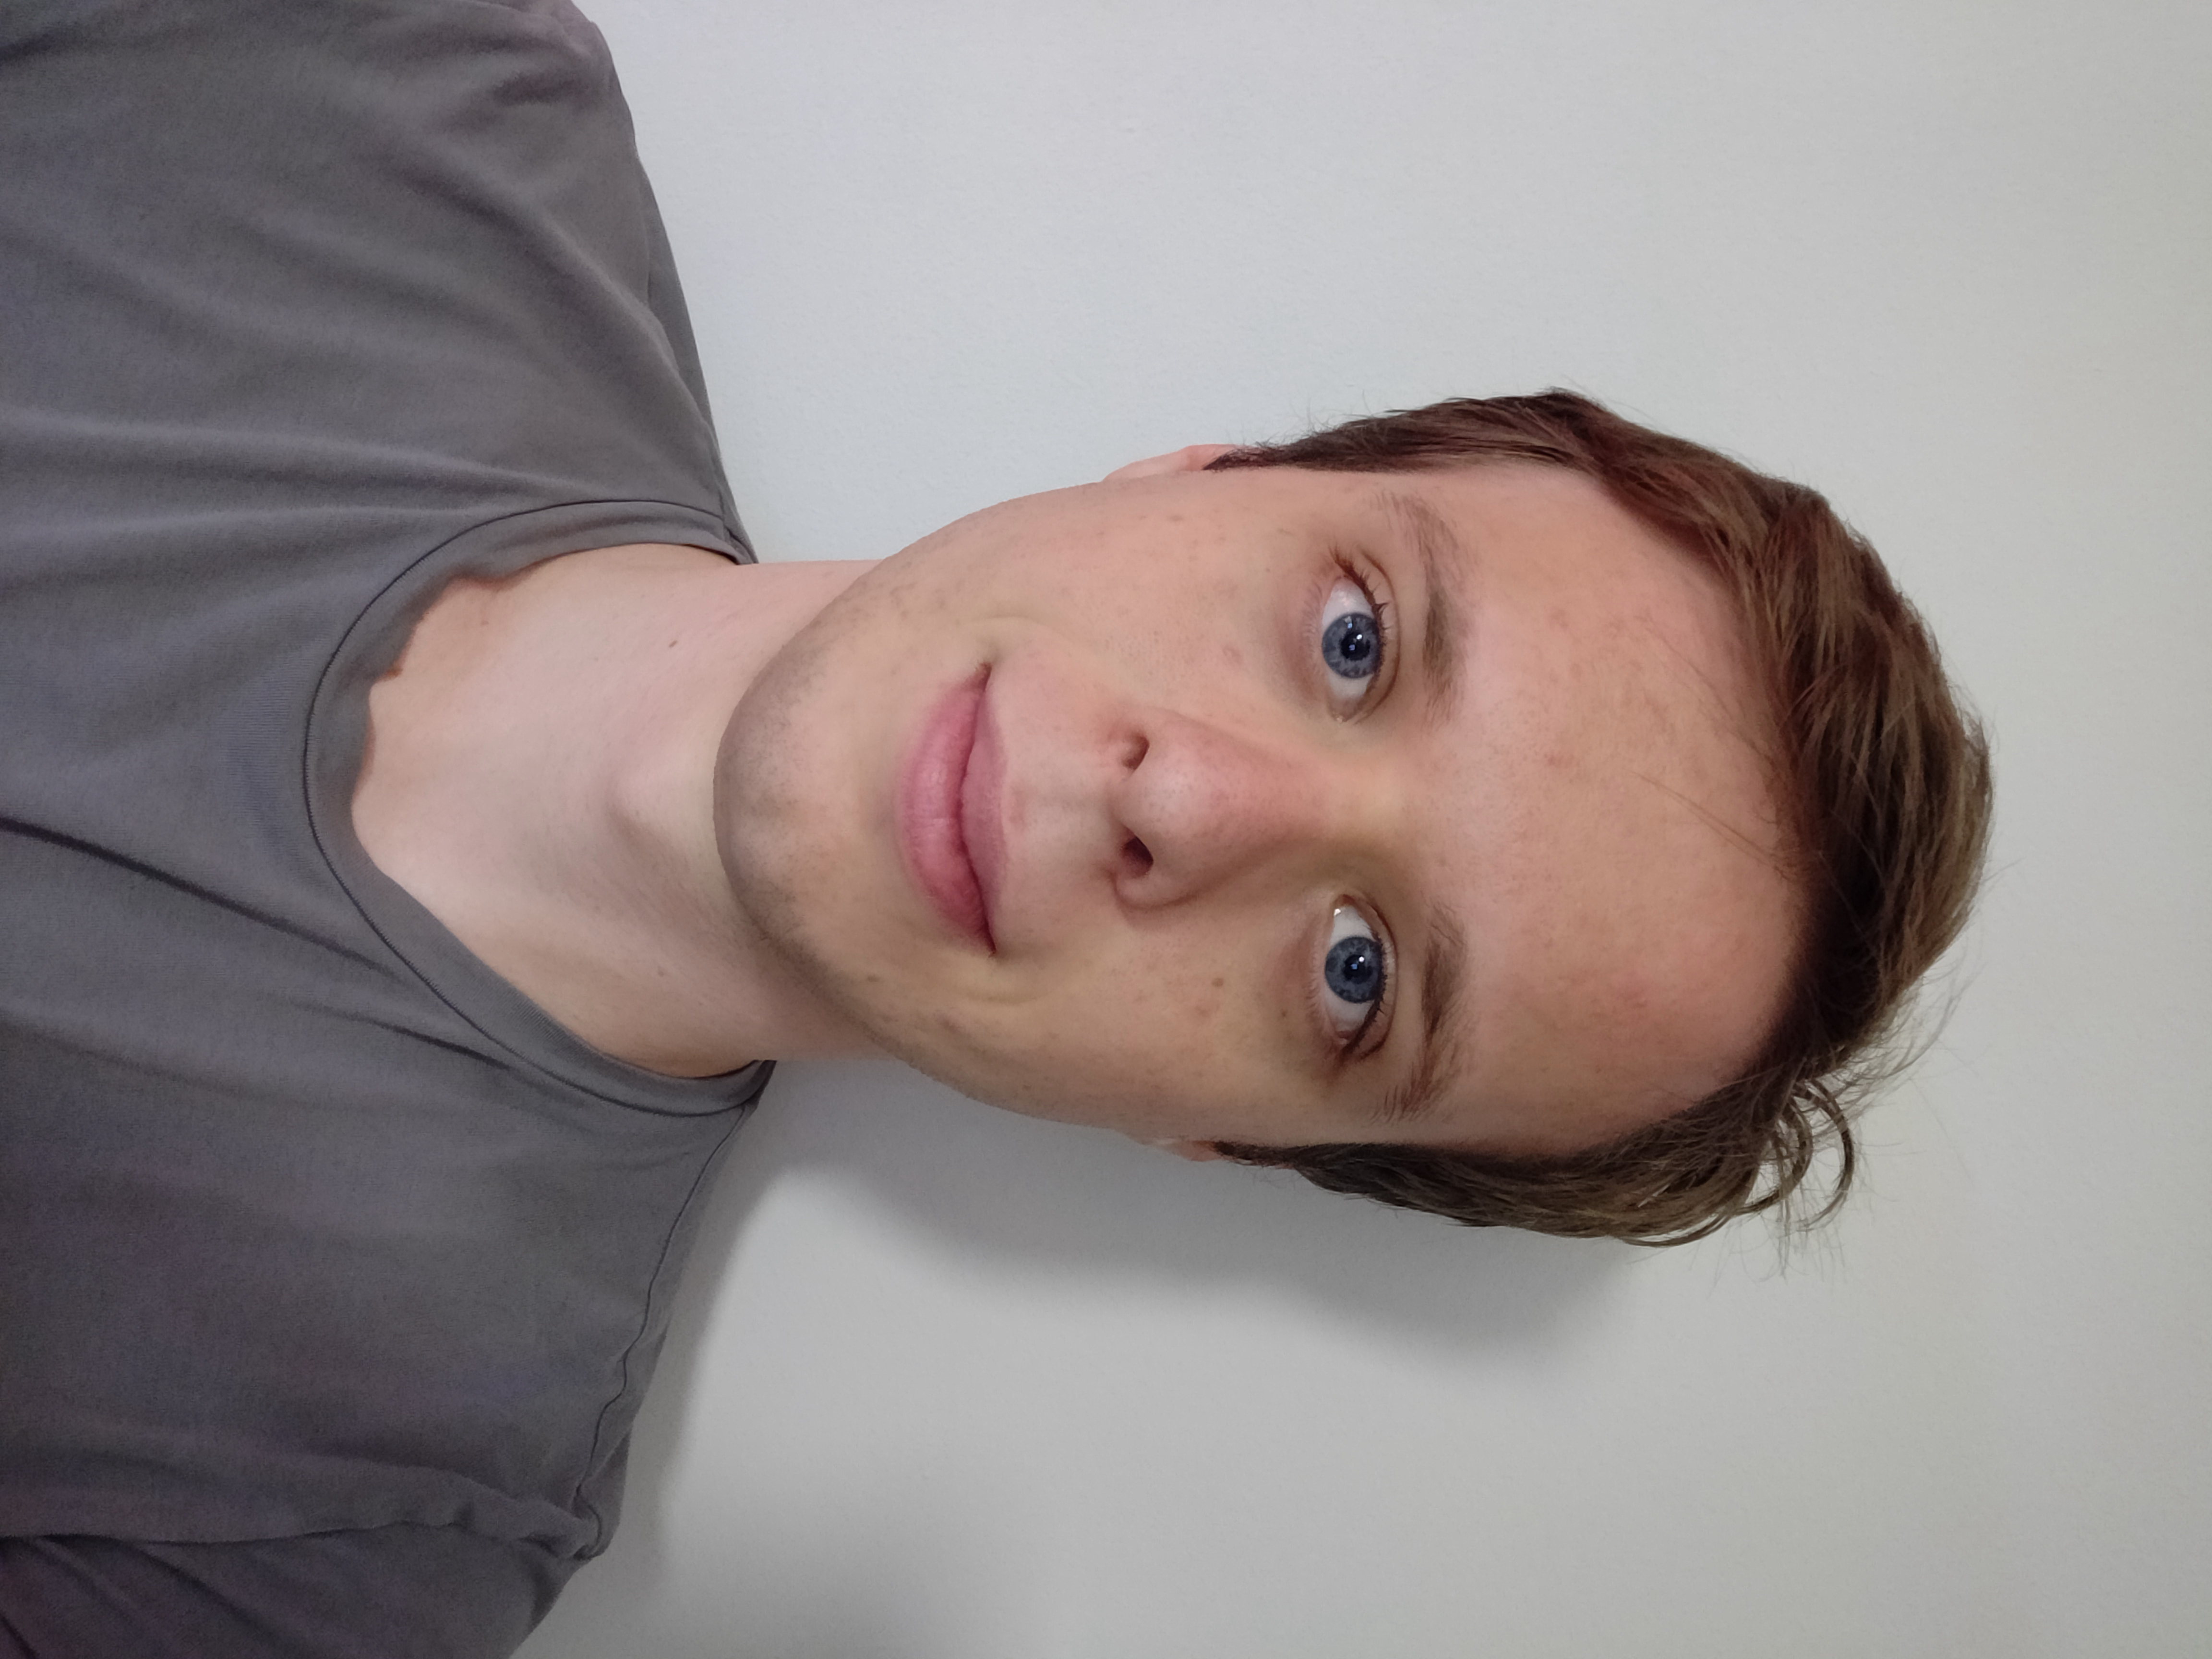
\includegraphics[width=1\columnwidth, angle=0]{photo-Mattia}
	\vspace{-7cm}
\end{figure}

\begin{flushright}\small
	Mattia Rubini \\
	mattia.rubini@gmail.com \\
	+39 329 617 1153 \\
	Account: 
	\href{https://github.com/Mot93}{GitHub}\\
	Account:
	\href{https://gitlab.com/mattia.rubini}{GitLab}\\
	Account:
	\href{https://stackoverflow.com/users/6875945/mattia-rubini}{Stack Overflow}
\end{flushright}\normalsize
\framebreak


% Right frame
%%%%%%%%%%%%%%%%%%%%
\Huge\bfseries {\color{RoyalBlue} Rubini Mattia} \\
\Large\bfseries  Developer - Laureando in Ing. Informatica \\

\normalsize\normalfont

% About me
\CVSection{Presentazione}
    Sono un laureando in Informatica all'università di Bologna, e mi dedico a progetti di programmazione dall'età di 14 anni.\\
	In tutto quello che faccio, cerco sempre di migliorarmi e di imparare cose nuove.
	Tutti i progetti realizzati fino ad oggi sono frutto sia del mio lavoro da autodidatta che degli approfondimenti acquisiti nel corso dei miei studi di laurea.
	\\Questo curriculum è stato realizzato con \LaTeX, un linguaggio markup:
	il sorgente si trova presso il mio \href{https://github.com/Mot93/CV-Mattia-Rubini}{account gitHub}\\
\Sep


% Experience
\CVSection{Esperienze}

\CVItem{Giu 2019 - ad oggi, Impiegato persso MAIS Family Office}\\
	Impiegato presso il MAIS family office ho incominciato il percorso di System Integrator. 
	Finita la mia formazione, ho incominciato ad espandermi in altri ruoli. 
	Mi sono appassionato della figura del Network Engineer, System Administrator e Data Scientist.
	Aiutando i miei colleghi impiegati in questi settori, ho acquisito nuove conosceze e sono cresciuto anche nei loro ambiti.

\SmallSep

\CVItem{Feb 2017 - Mag 2017, Postfix Calculator (app Android)}\\
	Ho imparato a programmare app usando android studio, Java e XML. 
	A seguire ho pubblicato una app android \href{https://play.google.com/store/apps/details?id=postfixcalculator.mattiarubini.com.postfixcalculator}{ Postifix Calculator}.
	Il codice sorgente è pubblico su \href{https://gitlab.com/mattia.rubini/PostfixCalculator}{gitlab}
\SmallSep

\CVItem{Nov 2016 - Feb 2017, Wordpress (sito personale)}\\
	Ho imparato a fare siti con wordpress. 
	Con queste nozioni ho fatto il mio sito personale. Il codice sorgente è disponibile su \href{https://github.com/Mot93/MattiaRubini-com-wordpress-theme}{github}.
\Sep

% Education
\CVSection{Formazione}

\CVItem{2020 - ad oggi, Laureando in Informatica}\\
	Nel 2020 ho deciso di cambiare nuovamente facoltà, per focalizzarmi sullo studio dell'informatica e di abbandonare la parte hardware che viene proposta ad ingegneria,
	presso l'Alma Mater Studiorum di Bologna.
\SmallSep

\CVItem{2017 - 2020, Laureando in Ingegneria Informatica}\\
	Nel 2017 ho deciso di cambiare facoltà, per focalizzarmi sullo studio dell'informatica, presso l'Alma Mater Studiorum di Bologna.
\SmallSep

\CVItem{2014 - 2015, Borsa di studio a Shanghai}\\
	Vincitore della borsa di studio di Ingegneria per l'overseas di un anno a Shanghai, presso la Tongji University.
\SmallSep

\CVItem{2013 - 2016, Laureando in Ingegneria dell'Automazione}\\
	% Bologna è a capo per non rompere il file
	\textbf{Interrotto, per trasferimento ad Informatica.}\\
	Iscritto presso il corso di laurea di Ingegneria dell'Automazione presso l'Alma Mater Studiorum di Bologna.
	Superati 15 esami. 
\SmallSep

% reset boundaries when going on a new page
\clearpage
\framebreak
\framebreak

\CVItem{2007 - 2013, Diploma}\\
	Diplomato presso il liceo scientifico Niccolò Copernico di Bologna.\\
	Indirizzo di studi MAXI (potenziamento di liceo scientifico, su materie: matematica, fisica, programmazione e scienze).\\
	Tale indirizzo insegna a programmare fin dai primi anni. 
\Sep

% Skills
\CVSection{Competenze}
\CVItem{Competenze informatiche avanzate}
\begin{multicols}{3}
\begin{compactitem}[\color{RoyalBlue}$\circ$]
	\item Docker
	\item Python 
	\item HTML
	\item CSS
	\item Javascript
	\item git
	\item shell
	\item bash
	\item SQL
	\item Rust
	\item Apparecchiature \\ Ubiquity
\end{compactitem}
\end{multicols}
\SmallSep

\CVItem{Competenze informatiche}
\begin{multicols}{3}
\begin{compactitem}[\color{RoyalBlue}$\circ$]
	\item Java
	\item Ansible
	\item Wordpress
	\item Django
	\item \LaTeX
	\item Pascal
	\item Windows
	\item Linux
	\item MacOS
	\item Raspberry Py
	\item Arduino
	\item Assemblamento\\computer
	\item Jupyter
	\item BMS
	\item KNX
\end{compactitem}
\end{multicols}
\SmallSep

\CVItem{Lingue conosciute}
\begin{multicols}{3}
\begin{compactitem}[\color{RoyalBlue}$\circ$]
	\item Italiano\\(madrelingua)
	\item Francese\\(madrelingua)
	\item Inglese (avanzato)
\end{compactitem}
\end{multicols}
\Sep 

\CVSection{Motivazione}
	Non mi spavento facilmente davanti le avversità.
	Per non fermarmi davanti il primo ostacolo, a 16 anni ho imparato l'inglese (livello avanzato) per accedere a più materiale possibile.
	\\Questa mia indole, mista alla mia passione per l'infromatica, mi ha permesso conoscere ed approfondire numerosi strumenti 
	grazie ai quali ho realizzato i numerosi progetti esposti sui miei account.

\CVSection{Altre esperienze}
	Membro del Rotaract Club Bologna Valle del Savena.
	\\System administrator del distretto Rotaract 2072.
	\\Assemblo computer per uso personale, amici e familiari.
	\\Ho progettato e realizzato la rete della mia abitazione, usando prodotti professionali Ubiquity.
	\\Il mio interesse per Raspberry Pi e Arduino ha trovato applicazione sia nella supervisione degli apparati tecnologici del MAIS family office, sia per la mia bitazione.
	\\Vacanza studio-lavoro di un mese con attività di volontariato per la ripopolazione della vegetazione in Islanda.
	\\Vacanza studio-lavoro di un mese con attività di volontariato per la preparazione di una struttura dedicata a ragazzi disadattati in Inghilterra.
	\\Attività di volontariato presso circolo Ancescao di Corticella in qualità di barista.
	\\Lavoro estivo in qualità di magazziniere in struttura a temperatura controllata, per generi alimentari.
\Sep

% References
%\CVSection{References}
%References upon request.

%%%%%%%%%%%%%%%%%%%%%%%%%%%%%%%%%%%%%
% End document
%%%%%%%%%%%%%%%%%%%%%%%%%%%%%%%%%%%%%
\end{document}